\documentclass[9pt,twocolumn,twoside]{pnas-new}
\usepackage{float}
\usepackage{multicol}
\usepackage{subcaption}
% Use the lineno option to display guide line numbers if required.

\templatetype{pnasresearcharticle} % Choose template
% {pnasresearcharticle} = Template for a two-column research article
% {pnasmathematics} %= Template for a one-column mathematics article
% {pnasinvited} %= Template for a PNAS invited submission

\begin{document}
\title{Co-Authorship Practices in Computer Science and Psoriasis Medical Research Networks}

% Use letters for affiliations, numbers to show equal authorship (if applicable) and to indicate the corresponding author
\author[a,1]{Adhikari, Anweshan}
\author[a,1]{Cataldo, Frannie}
\author[a,1]{Liem, Josef}

\affil[a]{Middlebury College Department of Computer Science}

% Please give the surname of the lead author for the running footer
\leadauthor{Liem}

% Please add a significance statement to explain the relevance of your work
\significancestatement{Our comparative analysis reveals key insights of computer science and health science collaboration networks in terms of moderate degree assortativities. This pattern deviates significantly from random networks, suggesting intentional collaboration strategies. Additionally, network position explains about half the variance in academic success across both fields, with number of collaborators (degree) being the strongest predictor of impact. These findings offer a nuanced view of collaboration dynamics and may inform strategies for building effective research networks. }

% Please include corresponding author, author contribution and author declaration information
\authorcontributions{Frannie Cataldo contributed in aspects of machine learning analysis, CS network analysis, and drafting of these sections in the report and presentation. Josef Liem was responsible for the management of APIs for additional network metadata, analysis of psoriasis collaboration and citation research networks, and drafting of the corresponding methods and results in the paper and presentation. Anweshan Adhikari contributed to statistical significance testing over the psoriasis research network, as well as drafting of the introduction and discussion of the paper and presentation.}
\correspondingauthor{\textsuperscript{1} E-mail: jliem@middlebury.edu}

% At least three keywords are required at submission. Please provide three to five keywords, separated by the pipe symbol.
\keywords{Networks $|$ Co-authorship $|$ Collaboration}

\begin{abstract}
Studying scientific collaboration practices provides important insight into how impactful research is generated within academic disciplines. Using bibliometric datasets, we applied a network-based approach to analyzing and understanding co-authorship structures in medical research on psoriasis, and computer science (CS). We examined metrics such as degree assortativity, centrality, and cluster to asses author collaborations and their relationships with scholarly impact for metrics like relative citation ratio (RCR), NIH percentile, total citations for the health science, and h-index for computer science. We compared our metrics against null models generated through Chung-Lu and preferential attachment methods. Our analysis demonstrated that both the CS research and psoriasis research networks exhibited stronger degree assortativity than by chance, suggesting selective patterns of collaboration, largely clustered by nationality. Moreover, the collaboration centrality strongly correlated to previously mentioned metrics for author success. We further employed machine learning methods to quantify authors' publication success based solely on network structural features, which accounted for nearly 50\% of the variance in author impact. The number of collaborators emerged as the strongest individual predictor. These results offer critical insight into the underlying dynamics of collaboration among influential scientists in the fields of CS and medicine.
\end{abstract}

\dates{This manuscript was compiled on \today}


\maketitle
\thispagestyle{firststyle}
\ifthenelse{\boolean{shortarticle}}{\ifthenelse{\boolean{singlecolumn}}{\abscontentformatted}{\abscontent}}{}

\firstpage{5}
\section*{INTRODUCTION}
\dropcap{S}cientific collaboration has become increasingly prevalent across disciplines, with researchers forming complex networks of co-authorship that reflect the social and intellectual structure of their fields \cite{newman2004coauthorship}. Understanding these collaborative structures provides crucial insights into how scientific knowledge is created, disseminated, and advanced within academic communities. Co-authorship networks—where nodes represent researchers and edges represent joint publications—serve as valuable proxies for analyzing collaboration patterns and their relationship to research impact \cite{borner2005studying}. These networks often exhibit small-world properties, combining high clustering with short path lengths that facilitate efficient knowledge transfer \cite{watts1998collective}.
\newline

 \noindent The structural properties of scientific collaboration networks vary significantly across disciplines, reflecting different research cultures, methodologies, and organizational frameworks \cite{wagner2011approaches}. While previous studies have examined co-authorship networks in various fields individually \cite{gonzalez2015evolution, newman2004coauthorship}, less attention has been given to direct comparative analyses between domains with distinctly different collaborative traditions, such as computer science and health sciences.
 \newline
 
\noindent Recent advances reveal universal principles governing collaboration networks: researchers exhibit persistent individual "preferentiality parameters" determining whether they focus intensively on few collaborators or distribute efforts broadly \cite{iniquez2023universal}; and collaboration shows diminishing returns where increasingly large teams are required to achieve comparable citation gains \cite{lariviere2015team}. These findings suggest that effective collaboration networks must balance individual networking preferences with evolving team size requirements for impact.
\newline

 \noindent This study addresses how co-authorship networks in health and computer science domains differ in their structural properties, collaboration patterns, and researcher success factors, and to what extent these observed patterns deviate from random chance. We hypothesize that domain-specific practices influence both network topology and the relationship between network position and scholarly impact. We employ network science metrics including degree assortativity and Kendall's Tau correlation, comparing observed networks against null models including Chung-Lu random graphs and preferential attachment models \cite{barabasi2002evolution, 
jeong2003measuring, Litvak}.
\newline

 \noindent The relationship between network position and scholarly success represents a particularly intriguing aspect of this study. While conventional wisdom suggests that collaborating with highly-cited researchers enhances one's academic impact, the extent to which network features can predict research outcomes remains incompletely understood \cite{abbasi2011identifying, yan2012scholarly}. For health science researchers, we analyze correlations between network centrality and field-normalized impact metrics such as the Relative Citation Ratio (RCR) \cite{hutchins2016relative}, which provides a sophisticated measure of article influence adjusted for disciplinary citation patterns. For computer science researchers, we examine relationships between network position and traditional bibliometric measures including h-index and total citations. Additionally, by applying machine learning techniques to network features such as degree, eigenvector centrality, and authorship status, we quantify their collective power in predicting researchers' h-index, using Shapley value analysis to determine feature importance \cite{rozemberczki2022shapley}.
\newline

\section*{METHODS}
\subsection*{Data}  
 We considered two networks in our analysis; the co-authorship network of medical researchers studying psoriasis, and the co-authorship network of researchers in computer science. The network of medical researchers consisted of 48,964 author nodes and 211,540 collaboration edges, whereas the network of CS researchers contained 402,392 author nodes and 1,234,019 collaboration edges (Table 1 \& 2).
 \newline

 \noindent To obtain information on the number of citations, the first author, the last author, and other success metrics of the paper in the psoriasis network, we cross-referenced the PMIDs and the author names through the NIH iCite and E-Utilities APIs (Figure 3). For each author, the average number of citations, average NIH percentile, and other nontotal metrics (i.e. not total citations), we averaged over the metrics of each paper included in the network. Finally, we plotted the logarithmic scale degree sequence over both networks to understand whether they followed a power-law degree distribution. For the CS network, the academic title (professor, postdoc, student, or unknown), total number of citations, and h-index were author metrics already provided in the dataset. 
\begin{table}[H]
\centering
\caption{Summary statistics for the psoriasis co-authorship network}
\begin{tabular}{lr}
\midrule
Number of nodes & 48,964 \\
Number of edges & 211,540 \\
Number of components & 4,628 \\
Nodes in largest component & 35,886 \\
Edges in largest component & 191,335 \\
Highest degree node & 655 \\
\bottomrule
\end{tabular}

\addtabletext{Network overview for the psoriasis research co-authorship graph.}
\end{table}
 \begin{table}[H]
\centering
\caption{Summary statistics for the CS co-authorship network}
\begin{tabular}{lr}
\midrule
Number of nodes &  402,392\\
Number of edges & 1,234,019\\
Number of components & 133,159\\
Nodes in largest component & 258,949\\
Edges in largest component & 1,222,632\\
Highest degree node & 463
\\
\bottomrule
\end{tabular}

\addtabletext{Network overview for the CS research co-authorship graph.}
\end{table}
\begin{table}[H]
\centering
\caption{Significance of given author/paper metrics}
\begin{tabular}{>{\raggedright\arraybackslash}p{0.4\linewidth}>{\raggedright\arraybackslash}p{0.5\linewidth}}
\midrule
RCR&  Field and time normalized citation rate of a given paper\\
NIH percentile& Percentile for outperformance of other papers in the field\\
h-index& Author-level productivity and impact of citations for publications\\
First author& Conventionally the researcher making the greatest contribution\\
Last author& Conventionally the supervisor or principle investigator\\
\end{tabular}

\addtabletext{Author and paper metrics as well as their significance in the context of research\cite{iCite2019}.}
\end{table}

\subsection*{Node Centrality} 
In our analysis, we considered the eigenvector centrality as a measure of node importance in each of our networks. Formally, the eigenvector centrality \( \mathbf{x} \) is defined as the solution to the equation $\mathbf{A} \mathbf{x} = \lambda \mathbf{x}$, where \( \mathbf{A} \) is the adjacency matrix of the network, \( \lambda \) is the largest eigenvalue of \( \mathbf{A} \), and \( \mathbf{x} \) is the corresponding eigenvector. Each component \( x_i \) of \( \mathbf{x} \) represents the centrality score of author \( i \), indicating that an author is important if it they are collaborating with many or other important authors.
\newline

\noindent In the psoriasis network, we ran a Spearman's rank correlation of author eigenvector centrality against the number of collaborators (degree centrality), the status of last authorship, first authorship, total number of publications, total citations, average number of citations, and average NIH percentile. We justified the use of a non-parametric ranked correlation test on the basis that eigenvector centralities and other author metrics were not normally distributed. We conducted the same eigenvector centrality correlation analyses on the CS network, examining its relationship with academic title, total citations, h-index, and degree centrality. 

\subsection*{Degree Assortativity} 
In the psoriasis and CS collaboration networks, we assessed degree assortativity and Kendall's tau compared to null models to determine whether authors preferentially collaborated with researchers sharing similar levels of collaboration activity. Degree assortativity was defined as followed: 
\[
\text{Assortativity} = 
\left(
\begin{array}{c}
\text{Edges with} \\
\text{like degree}
\end{array}
\right)
-
\left(
\begin{array}{c}
\text{Expected same-} \\
\text{degree edges}
\end{array}
\right)
\]
\noindent As Litvak et al. pointed out, rank correlation tests were more appropriate when comparing assortativities between networks of different sizes, as it can influence the magnitude of the assortativity coefficient \cite{Litvak}.  Thus, we also included Kendall's tau for cross comparison of assortativities over the psoriasis and CS collaboration networks. For the psoriasis network, which follows a power-law degree distribution, assortativity values were sampled from both Chung–Lu and Barabási–Albert preferential attachment models to evaluate the significance of the observed assortativity against distributions generated by these random models. For the CS collaboration network, only the Chung-Lu model was considered, as the network did not meet the assumption of having a power-law distributed degree sequence.

\subsection*{Network Homophily} 
In the psoriasis collaboration network, we examining homophily of several author-level attributes by measuring assortativity. These attributes included node degree, total publications, average RCR, total citations, average citations, and average NIH percentile. Assortativity was computed for each attribute to determine whether authors preferentially collaborated with others of similar productivity, collaboration tendencies, or scientific impact. For the CS collaboration network, academic title, total citation, h-index, and degree homophily were also considered.

\subsection*{Community Detection}
Lastly, we applied the Louvain community detection algorithm on the psoriasis research network subset of authors with ten or more collaborations and publications. The Louvain method is a widely used, modularity-based algorithm for detecting communities in large networks. It operates by greedily optimizing the modularity score, a measure that quantifies the strength network clustering of nodes (in this case, authors) using the following equation: 
\[
Q = \frac{1}{2m} \sum_{i,j} \left[ A_{ij} - \frac{k_i k_j}{2m} \right] \delta(z_i, z_j)
\]

where:
\begin{itemize}
\setlength{\itemsep}{0pt}
\setlength{\parsep}{0pt}
    \item \( A_{ij} \) is the adjacency matrix element indicating the existence of a collaboration between authors \( i \) and \( j \),
    \item \( k_i = \sum_j A_{ij} \) is the sum of collaborations (or the degree) for author \( i \),
    \item \( m \) is the total number of edges in the network,
    \item \( z_i \) is the cluster assignment of node \( i \),
    \item \( \delta(z_i, z_j) \) is the Kronecker delta function, equal to 1 if \( i \) and \( j \) are in the same community, and 0 otherwise.
\end{itemize}

\newline

\noindent We then cross-referenced each author name, verifying matches with their existing publications/PMIDs in the ORCID database to  understand what similarities the collaborators shared in their professional backgrounds. 

\subsection*{Machine Learning}
In order to better understand some of the results gleaned from the analysis of the networks, we considered the computer science network authorship database and tried to predict the h-index of a given author based solely on some metadata and network characteristics.  For the inputs to our machine learning model, we considered the number of collaborators of the author represented by the degree of the node, the eigenvector centrality of the node, and the authorship status of the node, which was 0 for unknown, 1 for student, 2 for postdoc, and 3 for professor.  For the machine learning model, we utilized a multi-layer perceptron regressor, or MLPRegressor, with two layers and a hidden layer size of 100, the ReLU activation function, and the Adam optimizer.  To avoid spending too much time on the machine learning aspects of a network science project, much of the underlying math will not be explained and only the important aspects of the regressor will be discussed.  The ReLU activation function has the following definition: 
$$f(x) = max(0,x)$$
\noindent For the use case of predicting h-index, this function was perfect as the h-index of an author is always positive.  Thus, the activation function forces the network to only output valid h-indexes.  Another interesting factor of the multi-layer perceptron utilized here is the Adam optimizer.  This optimizer is a method for "stochastic optimization that only requires first-order gradients"\cite{kingma2017adammethodstochasticoptimization}.  Put simply, the Adam is an algorithm for optimizing the gradient of a function.  In our application, the loss function is the one we attempt to minimize.  This is accomplished by choosing parameters that, when plugged into the loss function, will yield the minimum possible loss and thus result in the best possible model.  When tested against other optimizers in multi-layer neural networks, Adam outperforms other optimizers and thus was chosen for this project\cite{kingma2017adammethodstochasticoptimization}. 

\subsection*{Shapley Values}
In order to try and understand what the most important factors in predicting the h-index are, Shapley values were implemented.  Shapley values "attribute to each feature the change in expected model prediction when conditioning on that feature"\cite{lundberg2017unifiedapproachinterpretingmodel}.  This means that, through Shapley values, we could attempt to understand how the model is predicting h-indexes and what values for each parameter as broadly indicative of a higher h-index.  The Shapley values were computed using the following formula\cite{lundberg2017unifiedapproachinterpretingmodel}:
\begin{equation}
\phi_i(f,x) = \sum_{z' \subseteq x'} \frac{|z'|!(M - |z'| - 1)!}{M!} \left[ f_x(z') - f_x(z' \setminus i) \right]
\label{eq:shapley}
\end{equation}
where $|z'|$ was the number of non-zero entries in $z'$, and $z' \subseteq x'$ represents all $z'$ vectors where the non-zero entries are a subset of the non-zero entries in $x'$.
 

 \section*{RESULTS}
\subsection*{Centrality Correlated with Author Success Metrics} Predictably, node degree, which is itself a centrality, shared the strongest correlation with eigenvector centrality of authors in the psoriasis research network (Figure 1). First and last authorship status had little correlation with centrality in the subset of authors with 10+ collaborations/publications, though a weak positive correlation was present over the network of all co-authors ($\rho$(48,962) = 0.23, p < 0.0001). This discrepancy likely reflects that authors with fewer publications are less established and play supporting roles. Other author/paper metrics such as total citations, average citations, and average NIH percentile for authors with 10+ papers/collaborators were strongly correlated with eigenvector centrality (Figure 1). 
\begin{figure}[H]
    \centering
        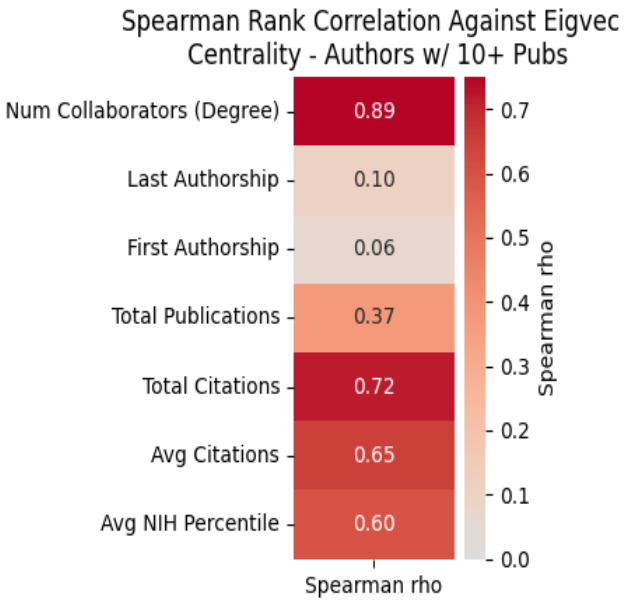
\includegraphics[width=0.25\textheight]{PsoriasisCentrality.png}
    \caption{Spearman's ranked correlation of eigenvector centralities in the psoriasis collaboration network against other author metrics. A non-parametric test was used as there could be no assumption of normally distributed metrics or centralities. Authors with 10+ publications were considered, as metrics were sparse for authors with fewer papers. All correlations were significant (p < 0.0001, d.f. = 48,962).}
    \label{fig:psoriasiscentrality}
\end{figure}
\noindent Likewise, in the network of CS researchers, number of collaborators/degree centrality was most highly correlated with eigenvector centrality, followed by author/paper metrics such as the total number of citations, and h-index (Figure 2). Academic titles showed little correlation with centrality, possibly due to many "unknown" classifications.

\begin{figure}[H]
    \centering
        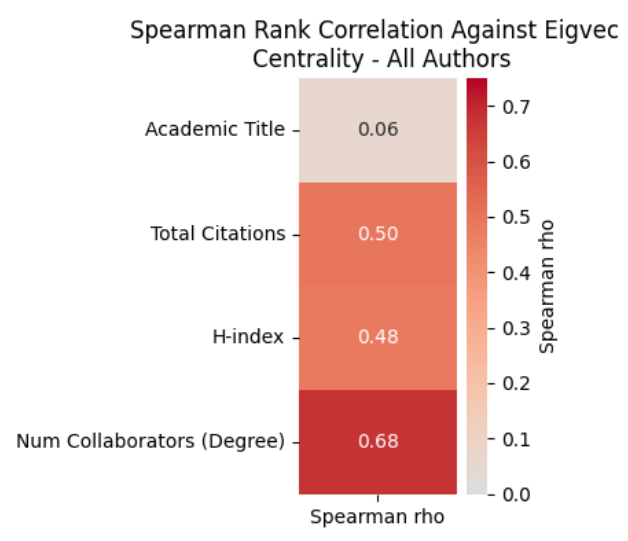
\includegraphics[width=0.25\textheight]{CSCentrality.png}
    \caption{Spearman's ranked correlation of eigenvector centralities in the CS collaboration research network against other author metrics. A non-parametric test was used as there could be no assumption of normally distributed metrics or centralities.}
    \label{fig:CScentrality}
\end{figure}
\subsection*{Collaborators Shared Similar Collaboration Levels} We then examined the degree assortativity and Kendall's tau for the psoriasis and CS networks. Degree assortativity of 0.17016 for the psoriasis network revealed a weakly assortative pattern (Table 4). That is, to some extent, authors tended to work with other authors who co-authored papers just as frequently. Likewise, a degree assortativity of 0.31082 for the CS network indicated moderate assortativity/like collaboration practices between collaborators (Table 5). When comparing both networks through Kendall's tau over author degrees, the CS network had a higher value overall (0.69997 vs. 0.45305) (Table 4 \& 5). Though, when factoring in the difference between their respective Chung-Lu models, Kendall's tau for the psoriasis research network was greater (0.13154 vs 0.07886). We did not consider the Barabási–Albert model for the CS network, as the degree distribution was not power-law distributed (Figure 4).
\begin{figure}[H]
    \centering
        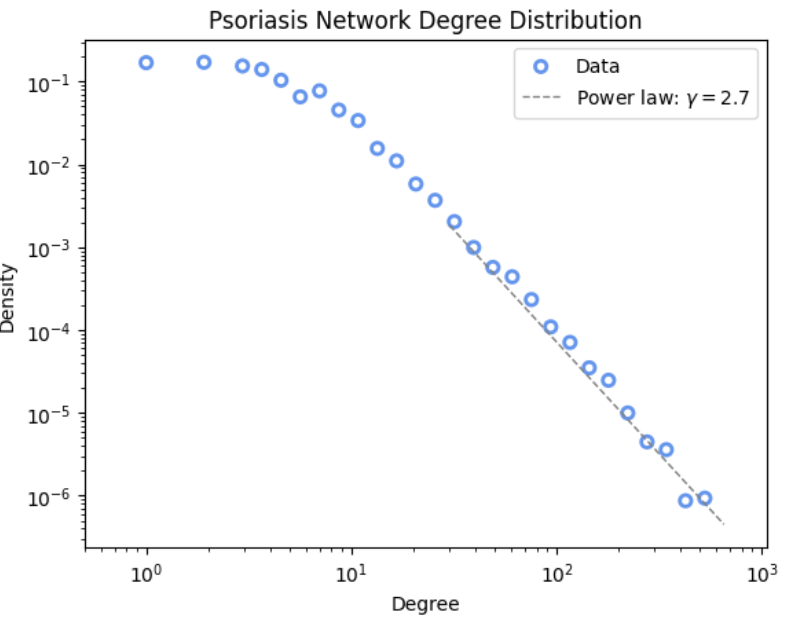
\includegraphics[width=0.32\textheight]{powerlawPsoriasis.png}
    \caption{Log-scale degree distribution of the psoriasis research network. This network appears to be power-law distributed.}
    \label{fig:powerlawPsoriasis}
\end{figure}
\begin{figure}[H]
    \centering
        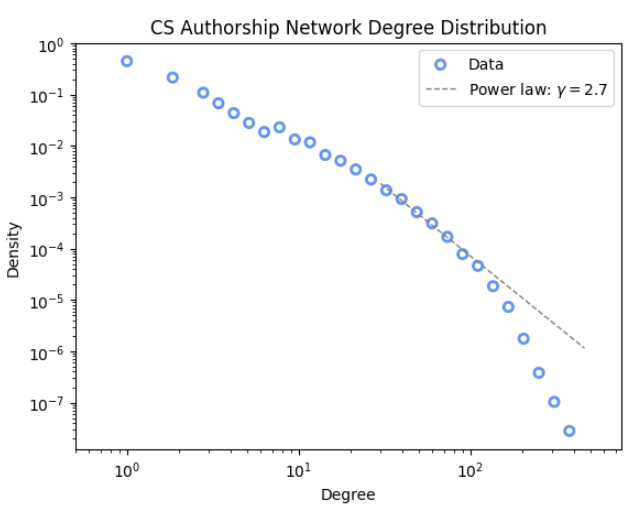
\includegraphics[width=0.32\textheight]{powerlawCS.png}
    \caption{Log-scale degree distribution of the psoriasis research network. This network is not scale free, as is evident in the tail end of higher degree.}
    \label{fig:powerlawCS}
\end{figure}
\renewcommand{\arraystretch}{0.75}
\begin{table}[htbp]
\centering
\caption{Psoriasis Network Degree Assortativity and Kendall's Tau Compared to Chung-Lu \& Barabási–Albert Models}
\setlength{\abovecaptionskip}{4pt}
\setlength{\belowcaptionskip}{4pt}

\begin{subtable}[t]{0.3\textwidth}
\centering
\caption{Mean Degree Assortativity (d.f. = 499)}
\setlength{\abovecaptionskip}{2pt}
\setlength{\belowcaptionskip}{4pt}
\begin{tabular}{>{\raggedright\arraybackslash}p{0.4\linewidth} >{\raggedleft\arraybackslash}p{0.25\linewidth} >{\raggedleft\arraybackslash}p{0.25\linewidth}}
\toprule
 & Mean & Std. Dev. \\
\midrule
Psoriasis Network & 0.17016 & n/a \\
Chung-Lu & -0.00098 & 0.00188 \\
Barabási–Albert & 0.00239 & 0.00135 \\
\bottomrule
\end{tabular}
\end{subtable}
\hfill
\begin{subtable}[t]{0.3\textwidth}
\centering
\caption{Mean Degree Kendall's Tau (d.f. = 499)}
\setlength{\abovecaptionskip}{2pt}
\setlength{\belowcaptionskip}{4pt}
\begin{tabular}{>{\raggedright\arraybackslash}p{0.4\linewidth} >{\raggedleft\arraybackslash}p{0.25\linewidth} >{\raggedleft\arraybackslash}p{0.25\linewidth}}
\toprule
 & Mean & Std. Dev. \\
\midrule
Psoriasis Network & 0.45305 & n/a \\
Chung-Lu & 0.32151 & 0.00301 \\
Barabási–Albert & 0.03318 & 0.00422 \\
\bottomrule
\end{tabular}
\end{subtable}

\vspace{0.1em}
\footnotesize
Degree assortativities and Kendall's tau values were sampled from distributions of Chung-Lu and Barabási–Albert models. The observed psoriasis network assortativity value was significantly different from those of the random models (one-sample t-test, d.f. = 499, p < 0.0001).
\label{tab:psoriasisassortativity}
\end{table}
\renewcommand{\arraystretch}{1.0}
\begin{table}[H]
\centering
\caption{CS Network Degree Assortativity and Kendall's Tau Compared to Chung-Lu Model}
\setlength{\abovecaptionskip}{4pt}
\setlength{\belowcaptionskip}{4pt}

\begin{subtable}[t]{0.3\textwidth}
\centering
\caption{Mean Degree Assortativity (d.f. = 49)}
\setlength{\abovecaptionskip}{2pt}
\setlength{\belowcaptionskip}{4pt}
\begin{tabular}{>{\raggedright\arraybackslash}p{0.4\linewidth} >{\raggedleft\arraybackslash}p{0.25\linewidth} >{\raggedleft\arraybackslash}p{0.25\linewidth}}
\toprule
 & Mean & Std. Dev. \\
\midrule
Psoriasis Network & 0.31082& n/a \\
Chung-Lu & 0.00392
& 0.00060\\
\end{tabular}
\end{subtable}
\hfill
\begin{subtable}[t]{0.3\textwidth}
\centering
\caption{Mean Degree Kendall's Tau (d.f. = 49)}
\setlength{\abovecaptionskip}{2pt}
\setlength{\belowcaptionskip}{4pt}
\begin{tabular}{>{\raggedright\arraybackslash}p{0.4\linewidth} >{\raggedleft\arraybackslash}p{0.25\linewidth} >{\raggedleft\arraybackslash}p{0.25\linewidth}}
\toprule
 & Mean & Std. Dev. \\
\midrule
Psoriasis Network & 0.69997
& n/a \\
Chung-Lu & 0.62111
& 0.00065
\\
\end{tabular}
\end{subtable}

\vspace{0.5em}
\footnotesize
Degree assortativities and Kendall's tau values were sampled from a distribution of Chung-Lu models. The observed psoriasis network assortativity value was significantly different from those of the random model (one-sample t-test, d.f. = 49, p < 0.0001). Barabási–Albert models were not considered for the CS network, as it was scale-free (Figure 4). 
\label{tab:psoriasisassortativity}
\end{table}
\subsection*{High Avg. RCR, Citations, NIH Percentile, and Degree Assortativities} Considering different measures of homophily over the psoriasis research collaboration network, authors had the greatest assortativity when examining average NIH Percentile, average citations per paper, and average RCR score (Figure 5). High assortativity over these metrics is to be expected, given that the average NIH percentile and citation scores of collaborating authors on papers are not entirely independent of one another. Though, given the lower assortativity for total number of citations for given authors, not all author/paper-based "success" metrics could be explained by this dependence alone. 
\begin{figure}[H]
    \centering
        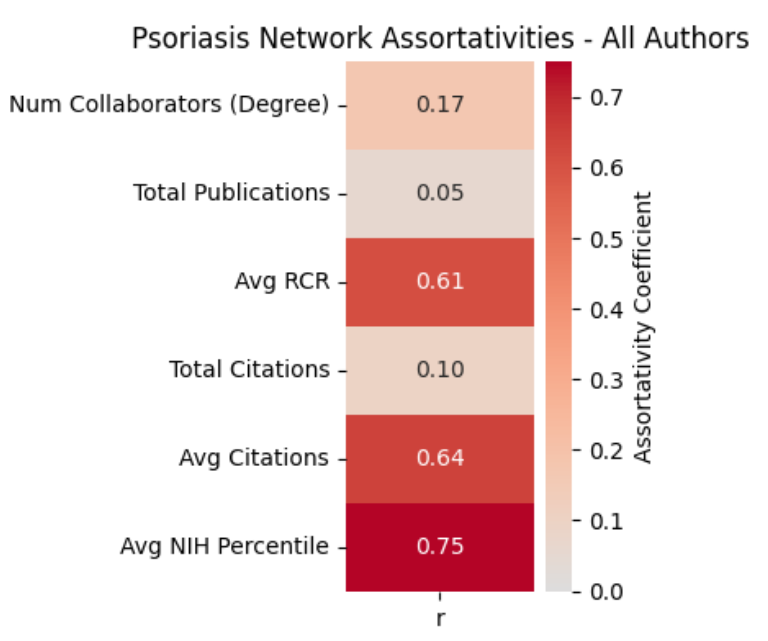
\includegraphics[width=0.25\textheight]{Homophily.png}
    \caption{Assortativity for author-level metrics in psoriasis network. Greatest homophily in NIH percentile and normalized success metrics. Scale: r=-1 (dis-assortative) < r=0 (non-assortative) < r=1 (assortative).}

    \label{fig:homophily}
\end{figure}

\subsection*{Collaborators Tended to Work with Others of Same National Origin or Country of Institutional Affiliation}
Comparing Louvain-detected communities among authors with 10+ publications and collaborations revealed that many clusters were composed of researchers from the same given country (Figure 6). In particular, U.S. and U.K.-based clusters often included individuals who had either trained or worked in those countries at some point in their careers. Thus, psoriasis medical research collaboration seemed to fall along institutional or national lines. Interestingly, researchers in Spain seem to form the most densely connected cluster of collaborating authors (Figure 6).
\begin{figure}[H]
    \centering
        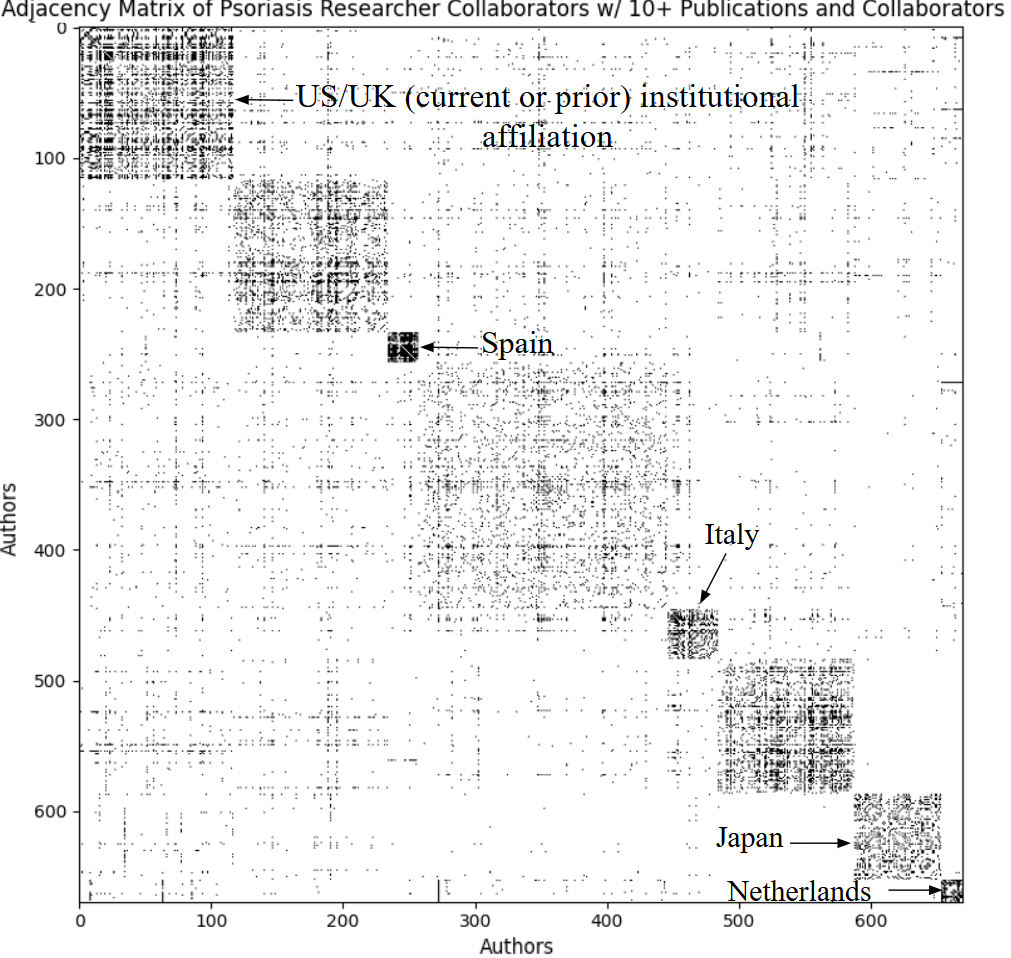
\includegraphics[width=0.35\textheight]{LouvainClustering.png}
    \caption{Adjacency matrix of psoriasis researchers (10+ publications/collaborations) showing co-authorship patterns. Louvain-detected clusters by country affiliation (ORCID-verified). Authors were predominantly physicians/dermatologists.}
    \label{fig:LouvainClustering}
\end{figure}

\subsection*{Collaboration Practices Largely Explained Variance in Models Quantifying h-index for the CS Network} 
After training the MLPRegressor on 80\% of the network nodes, the performance was evaluated on the remaining 20\% of the data.  The model achieved a $r^2$ score of $0.495$, which meant that the given parameters of the network (degree, eigenvector centrality, and authorship status) accounted for about half of the variance in quantifying the h-index. Applying Shapley values to our model, we could compute the following bee-swarm plot:
\begin{figure}[H]
    \centering
        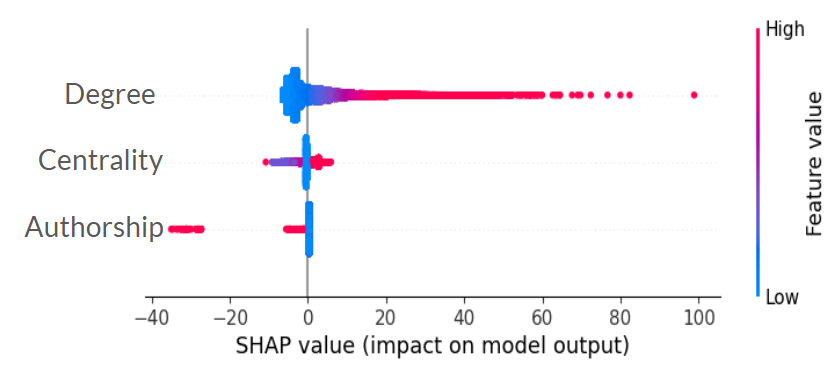
\includegraphics[width=0.35\textheight]{beeswarm.png}
    \caption{Beeswarm plot showing that the higher degree nodes had a positive impact on the predicted h-index. }
    \label{fig:beeswarm}
\end{figure}
\noindent 
This plot shows that higher degree nodes positively impacted predicted h-index, while high centrality was also predictive but with smaller effect. Shapley values for authorship were particularly interesting: unknown status (0) caused only small decreases since many unknowns were likely professors, professor status (3) provided small increases, while student (1) or postdoc (2) status greatly decreased expected h-index. This pattern makes sense given that students and postdocs have lower h-indices than professors, and since much data was unlabeled, unknowns could represent professors. Thus, the model predicted higher values for professors or unknowns and lower values for students or postdocs. Applied to a specific example, consider a node with degree 11, eigenvector centrality of 3.5e-7, and unknown authorship:

\begin{figure}[H]
    \centering
        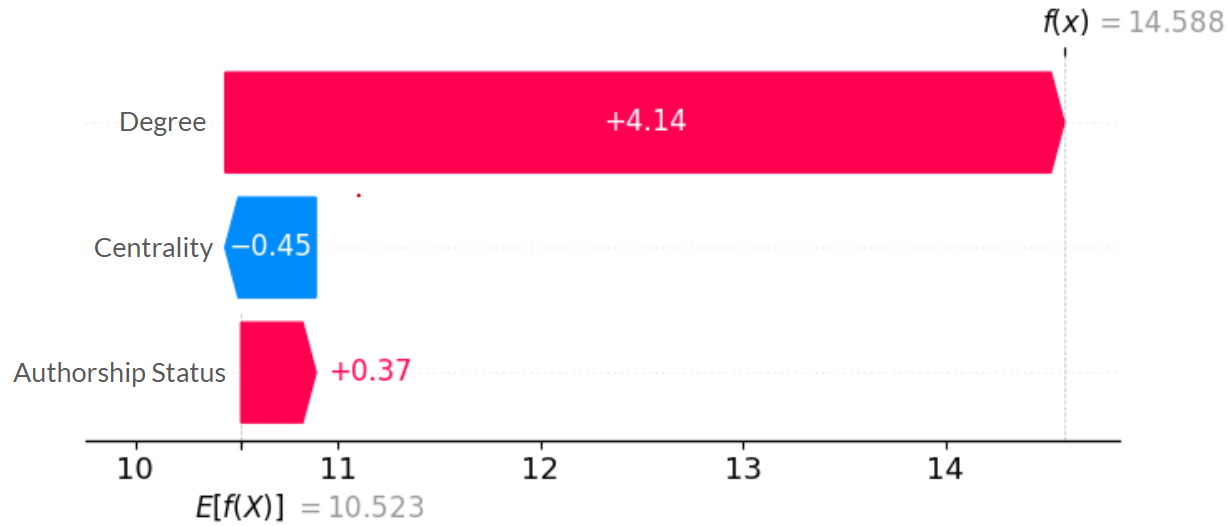
\includegraphics[width=0.37\textheight]{shap1.png}
    \caption{Shapley plot of h-index explained by given features of a collaborator.}
    \label{fig:shap1}
\end{figure}
\noindent Here, the results were quite similar to what was expected.  The high degree of 11 combined with a decently high eigenvector centrality caused our model to predict a higher than expected h-index, although the unknown authorship reduced it a bit.  This was a real author in the data with an actual h-index of 13 and the model predicted 14.588. 

  \section*{DISCUSSION}
\noindent Our findings challenge the assumption that scientific collaboration occurs randomly, revealing instead systematic patterns that suggest strategic network formation. Both networks showed that prolific collaborators work with other prolific collaborators, while occasional collaborators work with occasional collaborators. This aligns with social capital theory, where individuals invest in relationships that provide comparable resources and reciprocal benefits \cite{borner2005studying}. Moreover, the persistence of geographic clustering, particularly evident in our psoriasis network's nationality-based communities, supports the argument that structural properties of scientific collaboration networks vary significantly across disciplines, reflecting different research cultures and organizational frameworks \cite{wagner2011approaches}.
\newline

\noindent Perhaps most significant is our finding that network structural features explain approximately 50\% of the variance in h-index, directly validating and quantifying the predictions that network position correlates with scholarly success \cite{abbasi2011identifying,yan2012scholarly}. More importantly, our Shapley value analysis—extending the framework to academic networks \cite{rozemberczki2022shapley}—reveals that degree centrality dominates other network features, providing theoretically principled evidence that the number of collaborators, rather than their influence (eigenvector centrality), primarily drives academic impact. This finding aligns with the temporal inflation in collaboration documented by Larivière et al. \cite{lariviere2015team}, who showed that increasingly larger teams are required over time to achieve equivalent citation impact. This suggests that raw collaborative capacity (degree) outweighs the network prominence of one's collaborators (eigenvector centrality) in predicting research success.
\newline

\noindent However, our analysis has important limitations that suggest future research directions. First, comparing networks of vastly different sizes (48,964 vs. 402,392 nodes) may have biased our assortativity measures. Additionally, we treated all collaborations equally, but a two-author paper differs fundamentally from a 20-author paper. Weighted networks accounting for collaboration intensity and authorship roles represent important future extensions.
 \newline
 
\noindent More critically, we examined only co-authorship networks, missing how researchers influence each other through citations. While co-authorship has been established as a valuable proxy for collaboration patterns \cite{newman2004coauthorship}, the intersection between collaboration and citation networks remains unexplored—do researchers cite their collaborators more than strangers? Self-citation patterns are particularly relevant since excessive self-citing could artificially inflate the impact metrics (h-index, total citations) we used to measure success, potentially skewing our network-impact correlations. Future citation network analysis could employ algorithms like HITS to identify researchers who serve as both authorities (highly cited) and hubs (citing many others), complementing our centrality measures with citation-based influence patterns. Furthermore, our static network analysis overlooks temporal dynamics; as demonstrated in psoriasis research, cooperation patterns evolve over time \cite{gonzalez2015evolution}. Longitudinal analysis employing methods for measuring preferential attachment in evolving networks \cite{jeong2003measuring} could reveal whether collaboration strategies change as researchers advance in their careers.








\acknow{We would like to thank Professor Chodrow from the Middlebury College Computer Science Department for his teaching and assistance in determining the right direction and statistical analyses for this project.}

\showacknow{} % Display the acknowledgments section


%\bibsplit[1]
%Use \bibsplit to split the references from the body of the text. Value "[2]" represents the number of reference in the left column (Note: Please avoid single column figures & tables on this page.)

% Bibliography
\section*{BIBLIOGRAPHY}
\bibliography{bibliography}
\end{document}
